In this section, we present the performance model of applications
implemented using FDPS. As described in section \ref{sec:user}, the
calculation of a typical application written using FDPS proceeds in
the following steps

\begin{enumerate}
  \item Update the domain decomposition and exchange particles
    accordingly (not in every timestep).
  \item  Construct the local tree structure and exchange particles and
    superparticles necessary for interaction calculation.
  \item Construct the ``global'' tree.
  \item Perform the interaction calculation.
  \item Update the physical quantities of particles using the
    calculated interactions.
\end{enumerate}

In the case of complex applications which require more than one
interaction calculations, each of the above steps, except for the
domain decomposition, may be executed more than one time per one
timestep.

For a simple application, thus, the total wallclock time per one timestep should
be expressed as
\begin{equation}
  \label{eq:totalcost}
  T_{\rm step} =  T_{\rm dc}/n_{\rm dc}
               + T_{\rm lt}
               + T_{\rm exch}
               + T_{\rm icalc}
               + T_{\rm misc},
\end{equation}
where   $T_{\rm dc}$, $T_{\rm lt}$, $T_{\rm exch}$,
$T_{\rm icalc}$, and $T_{\rm misc}$ are the times for
domain composition and particle exchange, local tree construction,
exchange of particles and superparticles for interaction calculation,
interaction calculation, and other calculations such as particle
update, respectively. The term $n_{\rm dc}$ is the interval at which
the domain decomposition is performed.

In the following, we first construct the model for the communication
time. Then we construct models for each term of the right hand side of
equation~\ref{eq:totalcost}, and finally we compare the model with the
actual measurement presented in section
\ref{sec:total_time}.

\subsection{Communication model}
\label{sec:comm_model}

What ultimately determines the efficiency of a calculation performed
on a large-scale parallel machine is the communication overhead. Thus,
it is very important to understand what types of communication would
take what amount of time on actual hardware. In this section, we
summarize the characteristics of the communication performance of K
computer.

In FDPS, almost all communications are through the use of collective
communications, such as {\tt MPI\_Allreduce}, {\tt MPI\_Alltoall}, and
{\tt MPI\_Alltoallv}. However, measurement of the performance of these
routines for uniform message length is not enough, since the amount of
data to be transferred between processes generally depends on the
physical distance between domains assigned to those
processes. Therefore, we first present the timing results for simple
point-to-point communication, and then for collective communications.

Figure \ref{fig:pingpong} shows the elapsed time as the function of
the message length, for point-to-point communication between
``neighboring'' processes. In the case of K computer, we used
three-dimensional node allocation, so that ``neighboring'' processes
are actually close to each other in its torus network.

%For Cray XC30 we let the system to allocate nodes in its default
%mode.

We can see that the elapsed time can be fitted reasonably well as
\begin{equation}
\label{eq:Tp2p}
  T_{\rm p2p} = T_{\rm p2p,startup} + n_{\rm word}T_{\rm p2p,word},
\end{equation}
where $T_{\rm p2p,startup}$ is the startup time which is independent
of the message length and $T_{\rm p2p,word}$ is the time to transfer
one byte of message. Here, $n_{\rm word}$ is the length of the message
in units of bytes. On K computer, $T_{\rm p2p,startup}$ is 0.0101 ms
and $T_{\rm p2p,word}$ is $2.11 \times 10^{-7}$ ms per byte. For a
short message, there is a rather big discrepancy between the analytic
model and measured points, because for short messages K computer used
several different algorithms.


\begin{figure}
  \begin{center}
    \includegraphics[width=8cm]{figure/pingpong.eps}
  \end{center}
  \caption{
  
  Elapsed time for point-to-point communication as a function of size
  of message measured on K computer.

}
  \label{fig:pingpong}
\end{figure}



Figure \ref{fig:group_comm_a2a} shows the elapsed times for {\tt
MPI\_Alltoallv}. The number of processes $n_p$ is 32 to 2048. They are
again modeled by the simple form
\begin{equation}
\label{eq:wtime_group_comm}
  T_{\rm alltoallv} = T_{\rm alltoallv,\rm startup} + n_{\rm word}T_{\rm alltoallv,\rm word}, 
\end{equation}
where $T_{\rm \rm alltoallv,\rm startup}$ is the startup time and
$T_{\rm alltoallv,\rm word}$ is the time to transfer one byte of message.
We list these values in table \ref{table:alltoallv}.

\begin{table}
\caption{Time coefficients in equation (\ref{eq:wtime_group_comm})}
\begin{tabular}{|l|l|l|l|} \hline
                  & $n_p=32$ & $n_p=256$ & $n_p=2048$ \\ \hline
$T_{\rm alltoallv,startup}$ [ms] & 0.103 & 0.460 & 2.87 \\
$T_{\rm alltoallv,word}$ [ms/byte] & $8.25\times 10^{-6}$  & $9.13\times 10^{-5}$ & $1.32\times 10^{-3}$  \\ \hline
\end{tabular}
\label{table:alltoallv}
\end{table}


%In table \ref{table:domain_decomposition} we list these time coefficients.
%We can see that the agreement is reasonable. In
%table \ref{table:domain_decomposition} we list the values of these
%time constants.

The coefficients themselves in equation (\ref{eq:wtime_group_comm})
depend on the number of MPI processes $n_p$, as shown in
figures \ref{fig:group_comm_a2a_2}. They are modeled as
\begin{eqnarray}
\label{eq:alltoallv}
  T_{\rm alltoallv,startup} &=& \tau_{\rm alltoallv,startup} n_p, \\
  T_{\rm alltoallv,word} &=& \tau_{\rm alltoallv,word} n_p^{4/3}.
\end{eqnarray}
Here we assume that the speed to transfer message using {\tt
MPI\_Alltoallv} is limited to the bisection bandwidth of the system.
Under this assumption, $T_{\rm alltoallv,word}$ should be proportional
to $n_p^{4/3}$.  To estimate $\tau_{\rm alltoallv,startup}$ and
$\tau_{\rm alltoallv,word}$, we use measurements for message sizes of
8 bytes and 32k bytes. In K computer, we found that $\tau_{\rm
alltoallv,startup}$ is $0.00166$ ms and $\tau_{\rm alltoallv,word}$ is
$1.11 \times 10^{-7}$ ms per byte. If {\tt MPI\_Alltoallv} is limited
to the bisection bandwidth in K computer, $\tau_{\rm alltoallv,word}$
would be $5 \times 10^{-8}$ ms per byte. We can see that the actual
performance of {\tt MPI\_Alltoallv} on K computer is quite good.


%The two fittings to $T_{\rm alltoallv,startup}$ and $\tau_{\rm
%alltoallv,word}$ are reasonably well.

\begin{figure}
  \begin{center} 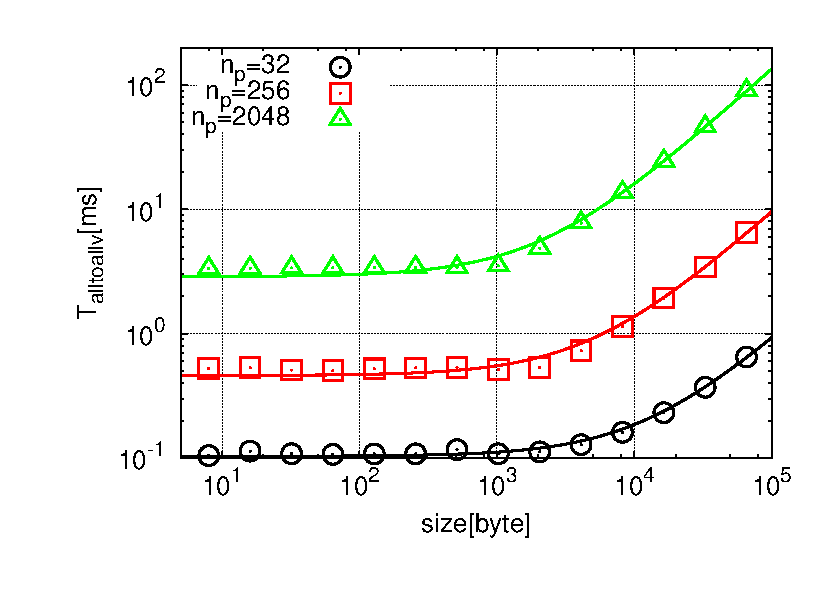
\includegraphics[width=8cm]{figure/comm/group_comm_a2a.eps}
  \end{center}
  \caption{
  
    Elapsed time of {\tt MPI\_Alltoallv} as a function of message size
    measured on K computer.

}
\label{fig:group_comm_a2a}
\end{figure}

\begin{figure}
  \begin{center}
  \includegraphics[width=8cm]{figure/comm/group_comm_a2a_2.eps}
  \end{center}
  \caption{
  
    Elapsed time of {\tt MPI\_Alltoallv} to send messeage of 8 bytes
    (circles) and 32k bytes (squares) as a function of the number of
    processes measured on K computer. Solid and dashed curves indicate
    the results for the message size of 8 bytes and 32k bytes,
    respectively.
    
} \label{fig:group_comm_a2a_2}
\end{figure}

%\begin{eqnarray}
%  T_{\rm type,startup} &=& \tau_{\rm type,startup} n_p \\
%  T_{\rm type,word} &=& \tau_{\rm type,word} n_p^{\alpha_{\rm type}}.
%\end{eqnarray}
%$T_{\rm alltoallv,word}$ and $T_{\rm allgatherv,word}$ are determined
%by the bisection and injection bandwidth. Thus $\alpha_{\rm
%alltoallv}$ is $4/3$ and $\alpha_{\rm allgatherv}$ is unity.

%Fitting the equations \ref{eq:alltoallv}, $\tau_{\rm
%alltoallv,startup}$ is $0.00166$ ms and $\tau_{\rm alltoallv,word}$ is
%0.00364 ms.


\subsection{Domain decomposition}

For the hierarchical domain decomposition method described in
section \ref{sec:decomposition}, the calculation time is expressed as

\begin{equation}
  \label{eq:dccost}
  T_{\rm dc} = T_{\rm dc,gather}
            +   T_{\rm dc,sort}
            +   T_{\rm dc,exch}
            +   T_{\rm dc,misc},
\end{equation}
where $T_{\rm dc,gather}$ is the time for the $(i,0,0)$ process to
collect sample particles, $T_{\rm dc,sort}$ is the time to sort sample
particles on the $(i,0,0)$ process, $T_{\rm dc,exch}$ is the time to
exchange particles after the new domains are determined, and $T_{\rm
dc,misc}$ is the time for remaining procedures such as initial
exchange of samples in $x$ direction, exchange of sample particles and
domain boundaries in $x$ direction, and broadcasting of the domain
boundaries in $y$-$z$ planes.

On the machines we so far tested, $T_{\rm dc,gather}$ and $T_{\rm
  dc,misc}$ are much smaller than $T_{\rm dc,sort}$ and $T_{\rm
  dc,exch}$. Therefore we consider these two terms only.

First, we consider the time to sort sample particles. Since we use the
quick sort, the term $T_{\rm dc,sort}$ is expressed as
%\begin{eqnarray}
%T_{\rm dc,sort} &=& \tau_{\rm qsort} \left[ 2n_{\rm smp} n_y n_z {\rm log} (n_{\rm smp} n_y n_z) + n_y n_{\rm smp} n_z {\rm log} (n_{\rm smp} n_z) \right], \\ 
%             &\sim& \tau_{\rm qsort} \left[ 2n_{\rm smp} n_p^{2/3} {\rm log} (n_{\rm smp} n_p^{2/3}) + n_p^{2/3} n_{\rm smp} {\rm log} (n_{\rm smp} n_p^{1/3}) \right],
%\end{eqnarray}
\begin{eqnarray}
T_{\rm dc,sort} &=& \tau_{\rm sort} \left[ 2n_{\rm smp} n_y n_z {\rm log} (n_{\rm smp} n_y n_z) + n_y n_{\rm smp} n_z {\rm log} (n_{\rm smp} n_z) \right] \\ 
             &\sim& \tau_{\rm dc,sort} n_{\rm smp}n_p^{2/3},
\end{eqnarray}
where $n_{\rm smp}$ is the average number of sample particles per
process, and $n_x$, $n_y$ and $n_z$ are the numbers of processes in x,
$y$ and $z$ direction. Here, $\tau_{\rm dc,sort} \sim {\rm log}(n_{\rm
smp}^3n_p^{5/3})\tau_{\rm sort}$. The first term expresses the time to
sort samples in $y$-$z$ planes with respect to $x$ and $y$
directions. The second term expresses that time to sort samples
respect to $z$ direction.

In order to model $T_{\rm dc,exch}$, we need to model the number of
particles which moves from one domain to another. This number would
depend on various factors, in particular the nature of the system we
consider. For example, if we are calculating the early phase of the
cosmological structure formation, particles do not move much in a
single timestep, and thus the number of particles moved between
domains is small. On the other hand, if we are calculating single
virialized self-gravitating system, particles move a relatively large
distances (comparable to average interparticle distance) in a single
timestep. In this case, if one process contains $n$ particles, half of
particles in the ``surface'' of the domain might migrate in and out
the domain. Thus, $O(n^{2/3})$ particles could be exchanged in this
case.

Figures \ref{fig:domain_decomposition_sort}, \ref{fig:domain_decomposition_exch}
and \ref{fig:domain_decomposition} show the elapsed time for sorting
samples, exchanging samples, and domain decomposition for the case of
disk galaxy simulations in the case of $n_{\rm smp}=500$ and $n \sim
5.3 \times 10^5$. We also plot the analytic models given by
\begin{eqnarray}
\label{eq:ddfit}
  T_{\rm dc} &\sim& T_{\rm dc,sort} + T_{\rm dc,exch} \\
             &=& \tau_{\rm dc,sort} n_{\rm smp} n_p^{2/3}
                 + \tau_{\rm dc,exch} \sigma \Delta t / \left<r\right> n^{2/3} b_p,
\end{eqnarray}
where $\tau_{\rm dc,sort}$ and $\tau_{\rm dc,exch}$ are the execution
time for sorting one particle and for exchanging one particle
respectively, $\sigma$ is the typical velocity of particles, $\Delta
t$ is the timestep and $\left<r\right>$ is the average interparticle
distance. For simplicity we ignore weak log term in $T_{\rm dc,sort}$
. On K computer, $\tau_{\rm dc,sort} = 2.67\times 10^{-7}$ second and
$\tau_{\rm dc,exch} = 1.42\times 10^{-7}$ second per byte. Note that
$\tau_{\rm dc,exch} \sim 672 T_{\rm p2p,word}$.

In figure \ref{fig:domain_decomposition_exch}, for small $n_p$, the
analytic model gives the value about 2 times smaller than the measured
point. This is because the measured values include not only the time
to exchange particles but also the time to determine appropriate
processes to send particles, while the analytic model includes only
the time to exchange particles. For small $n_p$, the time to determine
the appropriate process is not negligible, and therefor the analytic
model gives an underestimate.

%From figure \ref{fig:domain_decomposition_exch}, we can see that the
%left point is shifted upward from the fitted curve. This is because we
%used the least squares fitting and the right and center points are
%more highly weighted than the left one. In addition, we assumed that
%the particles are uniformly distributed, but in the simulation, we
%used the disk galaxy model (with high density contrast). The
%difference between the performance model and the simulation for this
%part is larger for smaller number of processes, because each
%computational domain has larger density contrast. Thus the left point
%is a bit far from the fitted curve.

%Note that $\tau_{\rm dc,sort} \sim {\rm log}(n_{\rm
%smp}^3n_p^{5/3})\tau_{\rm qsort}$.

%On K computer, $\tau_{\rm dc,sort} = 1.56\times 10^{-4}$ s and
%$\tau_{\rm dc,exch} = 5.53\times 10^{-5}$ s. Note that
%Figure \ref{fig:domain_decomposition} shows $T_{\rm dc}$ measured in
%K computer and its fitting curve using \ref{eq:ddfit} against the
%number of processes, in the case of $n_{\rm smp}=500$ and $n \sim
%5.3 \times 10^5$. In this case, we use $\tau_{\rm dc,sort} =
%1.56\times 10^{-4}$ ms and $\tau_{\rm dc,exch} = 8.65\times 10^{-7}$
%ms.

\begin{figure}
  \begin{center}
    \includegraphics[width=8cm]{figure/performance/domain_decomposition_sort.eps}
  \end{center}
  \caption{

Measured $T_{\rm dc,sort}$ and its analytic model as a function of
$n_p$, in the case of $n_{\rm smp}=500$ and $n \sim 5.3 \times 10^5$.

    }
  \label{fig:domain_decomposition_sort}
\end{figure}

\begin{figure}
  \begin{center}
    \includegraphics[width=8cm]{figure/performance/domain_decomposition_exch.eps}
  \end{center}
  \caption{

Measured $T_{\rm dc,exch}$ and its analytic model as a function of $n_p$, in
the case of $n_{\rm smp}=500$ and $n \sim 5.3 \times 10^5$.

    }
  \label{fig:domain_decomposition_exch}
\end{figure}

\begin{figure}
  \begin{center}
    \includegraphics[width=8cm]{figure/performance/domain_decomposition.eps}
  \end{center}
  \caption{

Measured $T_{\rm dc}$ and its analytic model as a function of $n_p$,
in the case of $n_{\rm smp}=500$ and $n \sim 5.3 \times 10^5$.

    }
  \label{fig:domain_decomposition}
\end{figure}

The analysis above, however, indicates that $T_{\rm dc,exch}$ is, even
when it is relatively large, still much smaller than $T_{\rm exch}$,
which is the time to exchange particles and superparticles for
interaction calculation (see section \ref{sec:exchnage_list}).

\subsection{Tree construction}

Theoretically, the cost of tree construction is $O(n{\rm log}n)$, and
of the same order as the interaction calculations itself. However, in
our current implementation, the interaction calculation is much more
expensive, independent of target architecture and the type of the
interaction. Thus we ignore the time for the tree constructions.


\subsection{Exchange of particles and superparticles}
\label{sec:exchnage_list}

For the exchange of particles and superparticles, in the current
implementation of FDPS, first each node constructs the list of
particles and superparticles (hereafter the exchange list) to be sent
to all other nodes, and then data are exchanged through a single call
to {\tt MPI\_Alltoallv}. The way the exchange list is constructed
depends on the force calculation mode. In the case of long-range
forces, usual tree traversal with a fixed opening angle $\theta$ is
performed. For the short-range forces, the procedure used depends on
the subtypes of the interaction. In the case of fixed or $j$-dependent
cutoff, the exchange list for a node can be constructed by a single
traversal of the local tree. On the other hand, for $i$-dependent or
symmetric cutoff, first each node constructs the $j$-dependent
exchange lists and sends them to all other nodes. Each node then
constructs the $i$-dependent exchange lists and sends them again.

The time for the construction and exchange of exchange list is thus
given by
\begin{equation}
  T_{\rm exch} = k_{\rm type}(T_{\rm exch,const}+T_{\rm exch,comm}).
  \label{eq:exchangecost}
\end{equation}

Here, $k_{\rm type}$ is an coefficient which is unity for fixed and
$j$-dependent cutoffs and two for other cutoffs. Strictly speaking,
the communication cost does not double for $i$-dependent or symmetric
cutoffs, since we send only particles which were not sent in the first
step. However, for simplicity we use $k=2$ for both calculation and
communication.

The two terms in equation (\ref{eq:exchangecost}) are then
approximated as
\begin{eqnarray}
  T_{\rm exch,const} &=& \tau_{\rm exch,const} n_{\rm exch,list}, \label{eq:exchange} \\
  T_{\rm exch,comm}(n_{\rm msg}) &=&  T_{\rm alltoallv}\left( n_{\rm exch,list}/n_{p} b_p \right), \label{eq:exchange_comm}
\end{eqnarray}

where $n_{\rm exch,list}$ is the average length of the exchange list
and $\tau_{\rm exch,const}$ is the execution time for constructing one
exchange list.  Figures \ref{fig:exchangeLET_nlist-wtime_const}
and \ref{fig:exchangeLET_nlist-wtime_exch} show the execution time for
constructing and exchanging the exchange list against the average
length of the list. Here, $b_p=48$ bytes for both short and long-range
interactions. From figure \ref{fig:exchangeLET_nlist-wtime_const}, we
can see that the elapsed time can be fitted well by equation
(\ref{eq:exchange}).  Here $\tau_{\rm exch,const}$ is $1.12 \times
10^{-7}$ second for long-range interaction and $2.31 \times 10^{-7}$
second for short-range interaction.

From figure \ref{fig:exchangeLET_nlist-wtime_exch}, we can see a large
discrepancy between measured points and the curves predicted from
equation (\ref{eq:exchange_comm}). In the measurement of the
performance of ${\tt MPI\_Alltoallv}$ in section \ref{sec:comm_model},
we used uniform message length across all processes. In actual use in
exchange particles, the length of the message is not
uniform. Neighboring processes generally exchange large messages,
while distant processes exchange short message. For such cases,
theoretically, communication speed measured in terms of average
message length should be faster. In practice, however, we observed a
serious degradation of performance. This degradation seems to imply
that the current implementation of ${\tt MPI\_Alltoallv}$ is
suboptimal for non-uniform message size.

\begin{figure}
  \begin{center}
    \includegraphics[width=8cm]{figure/performance/exchangeLET_nlist-wtime_const.eps}
  \end{center}
  \caption{
  
Time for the construction of the exchange list plotted against the
average length of the list, for the case of $n_p=2048$ and $n \sim
2.7 \times 10^5, 5.3 \times 10^5, 1.1 \times 10^6, 2.1 \times
10^6$. Circles and squares indicate the results for long-range and
short-range force, respectively. Solid and dashed curves are analytic
models [equation (\ref{eq:exchange})].

    }
  \label{fig:exchangeLET_nlist-wtime_const}
\end{figure}

\begin{figure}
  \begin{center}
    \includegraphics[width=8cm]{figure/performance/exchangeLET_nlist-wtime_exch.eps}
  \end{center}
  \caption{

Time for the communication of the exchange list against the average
length of the list per process, for the case of $n_p=2048$ and $n \sim
2.7 \times 10^5, 5.3 \times 10^5, 1.1 \times 10^6, 2.1 \times
10^6$. Circles and squares indicate the results for long-range and
short-range force, respectively. The curve is predicted from
equation (\ref{eq:exchange}).

    }
  \label{fig:exchangeLET_nlist-wtime_exch}
\end{figure}

In the following, we estimate $n_{\rm exch,list}$. If we consider a
rather idealized case, in which all domains are cubes containing $n$
particles, the total length of the exchange lists for one domain can
approximately be given by
\begin{equation}
\label{eq:n_list_long}
  n_{\rm exch,list} \sim \frac{14n^{2/3}}{\theta} + \frac{21\pi n^{1/3}}{\theta^2} + \frac{28\pi}{3\theta^3} {\rm log_2} \left\{ \frac{\theta}{2.8}\left[\left(nn_p\right)^{1/3} - n^{1/3}\right] \right\},
\end{equation}
for the case of long-range interactions and
\begin{equation}
\label{eq:n_list_short}
  n_{\rm exch,list} \sim \left( n^{1/3}-1+2\frac{r_{\rm cut}}{\left<r\right>} \right)^3-n,
\end{equation}
for the case of short-range interactions, where $r_{\rm cut}$ is the
average cutoff length and and $\left<r\right>$ is the average
interparticle distance. In this section we set $r_{\rm cut}$ so that
the number of particles in the neighbor sphere is to be 100. In other
words, $r_{\rm cut} \sim 3\left<r\right>$.

% and $n_{\rm ngb}$ is the number of the
%particles in the sphere with a radius of $r_{\rm cut}$.

In figure \ref{fig:exchangeLET_nlist-nsend}, we plot the list length
for short and long interactions against the average number of
particles. The rough estimate of equations (\ref{eq:n_list_long}) and
(\ref{eq:n_list_short}) agree very well with the measurements.

%Two curves are from
%equation \ref{eq:n_list_long} and \ref{eq:n_list_short}.

\begin{figure}
  \begin{center}
    \includegraphics[width=8cm]{figure/performance/exchangeLET_n-nsend.eps}
  \end{center}
  \caption{
  
The average length of the exchange lists for long-range interaction
(circles) and for short-range interaction (squares) as a function of
$n$, in the case of $\theta=0.4$ and $n_P=2048$. Solid and dashed
curves are predicted from equations (\ref{eq:n_list_long}) and
(\ref{eq:n_list_short}), respectively.

    }
  \label{fig:exchangeLET_nlist-nsend}
\end{figure}


\subsection{Tree traverse and interaction calculation}

The time for the force calculation is given by
\begin{equation}
T_{\rm icalc} = T_{\rm icalc,force} + T_{\rm icalc,const},
\end{equation}
where $T_{\rm icalc,force}$ and $T_{\rm icalc,const}$ are the time for
the force calculations for all particles and the tree traverses for
all interaction lists, respectively.

$T_{\rm icalc,force}$ and $T_{\rm icalc,const}$ are expressed as
\begin{eqnarray}
T_{\rm icalc,const} &=& \tau_{\rm icalc,const} n n_{\rm icalc,list} / n_{\rm grp}, \label{eq:wtime_force} \\
T_{\rm icalc,force}  &=& \tau_{\rm icalc,force} n n_{\rm icalc,list},
\end{eqnarray}
where $n_{\rm icalc,list}$ is the average length of the interaction
list, $n_{\rm grp}$ is the number of $i$ particle groups for modified
tree algorithms by \citet{1990JCoPh..87..161B}, $\tau_{\rm
icalc,force}$ and $\tau_{\rm icalc,const}$ are the time for one force
calculation and for constructing one interaction list.  In
figure \ref{fig:interaction_calc_nwalk-wtime}, we plot the time for
the construction of the interaction list as a function of $n_{\rm
grp}$. On K computer, $\tau_{\rm icalc,const}$ are $3.72\times
10^{-8}$ second for the long-range force and $6.59\times 10^{-8}$
second for the short-range force.

\begin{figure}
  \begin{center}
    \includegraphics[width=8cm]{figure/performance/interaction_calc_nwalk-wtime.eps}
  \end{center}
  \caption{

Time for the construction of the interaction list for long-range force
(circles) and short-range force (squares), for the case of $n \sim
5.3 \times 10^5$ and $\theta = 0.4$. Solid and dashed curves are the
analytic models for long-rage and short range forces, respectively
[equation (\ref{eq:wtime_force})].

    }
  \label{fig:interaction_calc_nwalk-wtime}
\end{figure}

The length of the interaction list is given by
\begin{equation}
\label{eq:nlist_long}
  n_{\rm icalc,list} \sim n_{\rm grp} + \frac{14n_{\rm grp}^{2/3}}{\theta} + \frac{21\pi n_{\rm grp}^{1/3}}{\theta^2} + \frac{28\pi}{3\theta^3} {\rm log_2} \left[ \frac{\theta}{2.8}\left\{\left(nn_p\right)^{1/3} - n_{\rm grp}^{1/3}\right\}\right]
\end{equation}
for the case of long-range interactions and
\begin{equation}
\label{eq:nlist_short}
  n_{\rm icalc,list} \sim \left( n_{\rm grp}^{1/3}-1+2\frac{r_{\rm cut}}{\left<r\right>} \right)^3,
\end{equation}
for the case of short-range interactions.

In figure \ref{fig:interaction_calc_ng-nlist}, we plot the length of
the interactions lists for long-range force and short-range force. We
can see that the length of the interaction lists can be fitted
reasonably well.

\begin{figure}
  \begin{center}
    \includegraphics[width=8cm]{figure/performance/interaction_calc_ng-nlist.eps}
  \end{center}
  \caption{

The average length of the interaction list for long-range force
(circles) and short-range force (squares), for the case of $n \sim
5.3 \times 10^5$ and $\theta = 0.4$. Solid and dashed curves are
analytic models for long-range [equation (\ref{eq:nlist_long})] and
short-range [equation (\ref{eq:nlist_short})] forces.

    }
  \label{fig:interaction_calc_ng-nlist}
\end{figure}

In the following, we discuss the time for the force calculation.  The
time for the force calculation for one particle pair $\tau_{\rm
icalc,force}$ has different values for different kinds of
interactions.  We plot $\tau_{\rm icalc,force}$ against $n_{\rm
icalc,list}$ for various $n_{\rm grp}$ in
figure \ref{fig:calc_force}. We can see that for larger $n_{\rm grp}$,
$\tau_{\rm icalc,force}$ becomes smaller. However, from equation
(\ref{eq:nlist_long}), large $n_{\rm grp}$ leads to large $n_{\rm
icalc,list}$ and the number of interactions becomes larger. Thus there
is an optimal $n_{\rm grp}$. In our disk-galaxy simulations in K
computer, the optimal $n_{\rm grp}$ is a few hundreds, and dependence
on $n_{\rm grp}$ is weak.

\begin{figure}
  \begin{center}
    \includegraphics[width=8cm]{figure/performance/calc_force.eps}
  \end{center}
  \caption{
  
  Time for the evaluation of one gravity force against $n_{\rm icalc,
  list}$ for various $n_{\rm grp}$.
  
    }
  \label{fig:calc_force}
\end{figure}




\subsection{Total time}
\label{sec:total_time}

Now we can predict the total time of the calculation using the above
discussions. The total time per one timestep is given by
\begin{eqnarray}
  T_{\rm step} &\sim& T_{\rm dc,sort}/n_{\rm dc} \nonumber
                  + k_{\rm type}\left( T_{\rm exch,const}+T_{\rm exch,comm} \right) \nonumber \\
                  &&+ T_{\rm icalc,force} + T_{\rm icalc,const} \label{eq:totalcost2} \\
             &\sim& \tau_{\rm dc,sort} n_{\rm smp} n_p^{2/3}/n_{\rm dc} \nonumber \\
                &&+ k_{\rm type}\left( \tau_{\rm exch,const} n_{\rm exch,list} + \tau_{\rm alltoallv,startup}n_p + \tau_{\rm alltoallv,word}n_{\rm exch,list}b_pn_p^{1/3} \right) \nonumber \\
                && + \tau_{\rm icalc,force} n n_{\rm icalc,list} \nonumber \\
                && + \tau_{\rm icalc,const} n n_{\rm icalc,list} / n_{\rm grp}.   \label{eq:totalcost3}
\end{eqnarray}
The time coefficients in equation (\ref{eq:totalcost3}) for K computer
are summarized in table \ref{table:time_coefficients}. In this section
we use $n_{\rm dc}=1$.

\begin{table}
\caption{Time coefficients in equation (\ref{eq:totalcost3}) for K computer.
$\tau_{\rm icalc,force}$ is the value for gravity.  }
\begin{tabular}{|l|l|} \hline
$\tau_{\rm alltoallv,startup}$ [s] & $1.66 \times 10^{-6}$ \\ 
$\tau_{\rm alltoallv,word}$ [s/byte] & $1.11 \times 10^{-10}$\\
$\tau_{\rm dc,sort}$ [s] & $2.67\times 10^{-7}$ \\ 
$\tau_{\rm exch,const}$ [s] & $1.12 \times 10^{-7}$ \\
$\tau_{\rm icalc,const}$ [s] & $3.72\times 10^{-8}$ \\
$\tau_{\rm icalc,force}$ [s] & $3.05\times 10^{-10}$ \\ \hline
\end{tabular}
\label{table:time_coefficients}
\end{table}

To see if the predicted time by equation (\ref{eq:totalcost3}) is
reasonable, we compare the predicted time and the time obtained from
the disk galaxy simulation with the total number of particles ($N$) of
550 million and $\theta = 0.4$. In our simulations, we use up to the
quadrupole moment. On the other hand, we assume the monopole moment
only in equation (\ref{eq:totalcost3}). Thus we have to correct the
time for the force calculation in equation (\ref{eq:totalcost3}). In
our simulations, the cost of the force calculation of the quadrupole
moment is two times higher than that of the monopole moment and about
75\% of particles in the interactions list are superparticles.  Thus
the cost of the force calculation in the simulation is 75\% higher
than the prediction. We apply this correction to equation
(\ref{eq:totalcost3}). In
figure \ref{fig:performance_model_strong_breakdown_comp}, we plot the
breakdown of the predicted time with the correction and the obtained
time from the disk galaxy simulations. We can see that our predicted
times agree with the measurements very well.

\begin{figure}
  \begin{center}
    \includegraphics[width=8cm]{figure/performance/performance_model_strong_breakdown_comp.eps}
  \end{center}
  \caption{
  
  Breakdown of the total time of the calculation per one timestep
  against $n_p$, for the case of $N=5.5\times 10^8$ , $n_{\rm
  smp}=500$, $\theta=0.4$ and $n_{\rm grp}=130$.
  
}
  \label{fig:performance_model_strong_breakdown_comp}
\end{figure}

In the following, we analyze the performance of the gravitational many
body simulations for various hypothetical computers. In
figure \ref{fig:performance_model_strong_breakdown}, we plot the
breakdown of the calculation time predicted using equation
(\ref{eq:totalcost3}) for the cases of 1 billion and 10 million
particles against $n_p$. For the case of 1 billion particles, we can
see that the slope of $T_{\rm step}$ becomes shallower for
$n_p \gtrsim 10000$ and increases for $n_p \gtrsim 30000$, because
$T_{\rm dc,sort}$ dominates. Note that $T_{\rm exch,comm}$ also has
the minimum value. The reason is as follows. For small $n_p$, $T_{\rm
alltoallv,word}$ is dominant in $T_{\rm exch,comm}$ and it decrease as
$n_p$ increases, because the length of $n_{\rm exch,list}$ becomes
smaller. For large $n_p$, $T_{\rm alltoallv,startup}$ becomes dominant
and it increases linearly. We can see the same tendency for the case
of 10 million particles. However, the optimal $n_p$, at which $T_{\rm
step}$ is the minimum, is smaller than that for 1 billion particles,
because $T_{\rm dc,sort}$ is independent of $N$.


\begin{figure}
  \begin{center}
    \includegraphics[width=8cm]{figure/performance/performance_model_strong_breakdown.eps}
  \end{center}
  \caption{
  
  Breakdown of the total time of the calculation per one timestep
  against $n_p$, for the case of $N=10^9$ (top panel) and $=10^7$
  (bottom panel), $n_{\rm smp}=500$, $\theta=0.4$ and $n_{\rm
  grp}=300$.
  
}
  \label{fig:performance_model_strong_breakdown}
\end{figure}

In figure \ref{fig:performance_model_strong_breakdown_x10}, we plot
the breakdown of the predicted calculation time for a hypothetical
computer which has the floating-point operation performance ten times
faster than that of K computer (hereafter X10). In other words,
$\tau_{\rm alltoallv,startup}$ and $\tau_{\rm alltoallv,word}$ are the
same as those of K computer, but $\tau_{\rm dc,sort}$, $\tau_{\rm
exch,const}$, $\tau_{\rm icalc,const}$ and $\tau_{\rm icalc,force}$
are ten times smaller than those of K computer. We can see that the
optimal $n_p$ is shifted to smaller $n_p$ for both cases of $N$ of 1
billion and 10 million, because $T_{\rm exch,comm}$ is unchanged.
However, the shortest time per timestep is improved by about a factor
of five.  If the network performance is also improved by a factor of
ten, we would get the same factor of ten improvement for the shortest
time per timestep. In other words, by reducing the network performance
by a factor of ten, we suffer only a factor of two degradation of the
shortest time.




\begin{figure}
  \begin{center} \includegraphics[width=8cm]{figure/performance/performance_model_strong_breakdown_x10.eps} \end{center} \caption{
  
The same as figure \ref{fig:performance_model_strong_breakdown}, but
for the floating-point operation performance ten times faster than K
computer.
  
}
  \label{fig:performance_model_strong_breakdown_x10}
\end{figure}

In figure \ref{fig:performance_model_strong_predict}, we plot
predicted $T_{\rm step}$ for three hypothetical computers and K
computer. Two of four computers are the same computer models we used
above. Another is a computer with the floating-point operation
performance hundred times faster than K computer (hereafter X100).
The last one is a computer of which the performance of the force
calculation is ten times faster than K computer (hereafter ACL). In
other words, only $\tau_{\rm icalc,force}$ is ten times smaller than
that of K computer.  This computer is roughly mimicking a computer
with an accelerator such as, GPU \citep{hamada2009novel},
GRAPE \citep{1990Natur.345...33S, 2003PASJ...55.1163M} and
PEZY-SC. Here we use the optimal $n_{\rm grp}$, at which $T_{\rm
step}$ is minimum, for each computers. For the case of $N=10^9$, the
optimal $n_{\rm grp} \sim 300$ for K computer and X10, $\sim 400$ for
X100 and $\sim 1600$ for ACL. For the case of $N=10^{12}$, the optimal
$n_{\rm grp}$ for K, X10, X100 is the same as those for $N=10^9$, but
$\sim 1800$ for ACL. The optimal value of $n_{\rm grp}$ for ACL is
larger than those of any other computers, because large $n_{\rm grp}$
reduces the cost of the construction of the interaction list.

From figure \ref{fig:performance_model_strong_predict}, we can see
that for small $n_p$, X10 and X100 are ten and hundred times faster
than K computer, respectively. However, for the case of $N=10^9$,
$T_{\rm step}$ of the values of X10 and X100 increase for $n_p \gtrsim
15000$ and $\gtrsim 7000$, because the $T_{\rm exch,comm}$ becomes the
bottleneck. ACL shows a similar performance to that of X10 up to
optimal $n_p$, because the force calculation is dominant in the total
calculation time. On the other hand, for large $n_p$, the performance
of ACL is almost the same as that of K computer, because ACL has the
same bottleneck as K computer has, which is the communication of the
exchange list.  On the other hand, for the case of $N=10^{12}$,
$T_{\rm step}$ is scaled up to $n_p \sim 10^5$ for all computers. This
is because for larger $N$ simulations, the costs of the force
calculation and the construction of the interaction list are
relatively higher than the communication of the exchange list. Thus
the optimal $n_p$ is sifted to larger value if we use larger $N$.



\begin{figure}
  \begin{center}
    \includegraphics[width=8cm]{figure/performance/performance_model_strong_predict.eps}
  \end{center}
  \caption{
  
Predicted total calculation time for three hypothetical computers and
K computer as a function of $n_p$, for the case of $n_{\rm smp}=500$,
$\theta=0.4$.  Top and bottom panels indicate the results of the case
for $N=10^{12}$ and $N=10^{9}$, respectively.
  
}
  \label{fig:performance_model_strong_predict}
\end{figure}

From figures \ref{fig:performance_model_strong_breakdown}
and \ref{fig:performance_model_strong_breakdown_x10}, we can see that
for large $n_p$, performance will be limited by $T_{\rm dc,sort}$ and
$T_{\rm exch,comm}$. Therefor, if we can reduce them further, we can
improve the efficiency of the calculation with large $n_p$. It is
possible to reduce the time for sort by applying the algorithm used in
$x$ direction to $y$ direction as well or setting $n_{\rm dc}$ to more
than unity. It is more difficult to reduce $T_{\rm exch,comm}$, since
we are using system-provided {\tt MPI\_Alltoallv}.

